\documentclass{article}

\usepackage{tikz}
\usetikzlibrary{patterns}

\definecolor{pantoneblack7}{RGB}{62,62,59}
\definecolor{pantone144}{cmyk}{0,0.5,1,0}
\definecolor{pantone289}{cmyk}{1,0.6,0,0.56}

\tikzset{candidate/.style={draw, align=center, rounded corners=0.1cm, fill=white}}
\tikzset{balanced/.append style={draw=pantone144, thick, fill=pantone144!40}}
\tikzset{todo/.append style={draw=pantone144, thick, pattern=north west lines, pattern color=pantone144!40}}
\tikzset{target/.style={align=center, draw, thick, fill=white}}

\usepackage{pgfplots}

% Code from Christian Feuersänger
% http://tex.stackexchange.com/questions/54794/using-a-pgfplots-style-legend-in-a-plain-old-tikzpicture#54834

% argument #1: any options
\newenvironment{customlegend}[1][]{%
    \begingroup
    % inits/clears the lists (which might be populated from previous
    % axes):
    \csname pgfplots@init@cleared@structures\endcsname
    \pgfplotsset{#1}%
}{%
    % draws the legend:
    \csname pgfplots@createlegend\endcsname
    \endgroup
}%

% makes \addlegendimage available (typically only available within an
% axis environment):
\def\addlegendimage{\csname pgfplots@addlegendimage\endcsname}

\usepackage[scaled]{berasans}
\renewcommand*\familydefault{\sfdefault}  %% Only if the base font of the document is to be sans serif
\usepackage[T1]{fontenc}

\usepackage{cleveref}

\begin{document}
\Cref{fig:balancing} shows the balancing dependencies in LLVM IR.
As the target for this thesis is to balance components of the actual processor, these are included as balancing milestones.
The prerequisites for a milestone are all types of variables that comprise it.
It is therefore balanced iff all prerequisites are balanced.

The implementation of hatched nodes is meant to be part of my thesis, but still open.

\begin{figure}[h]
  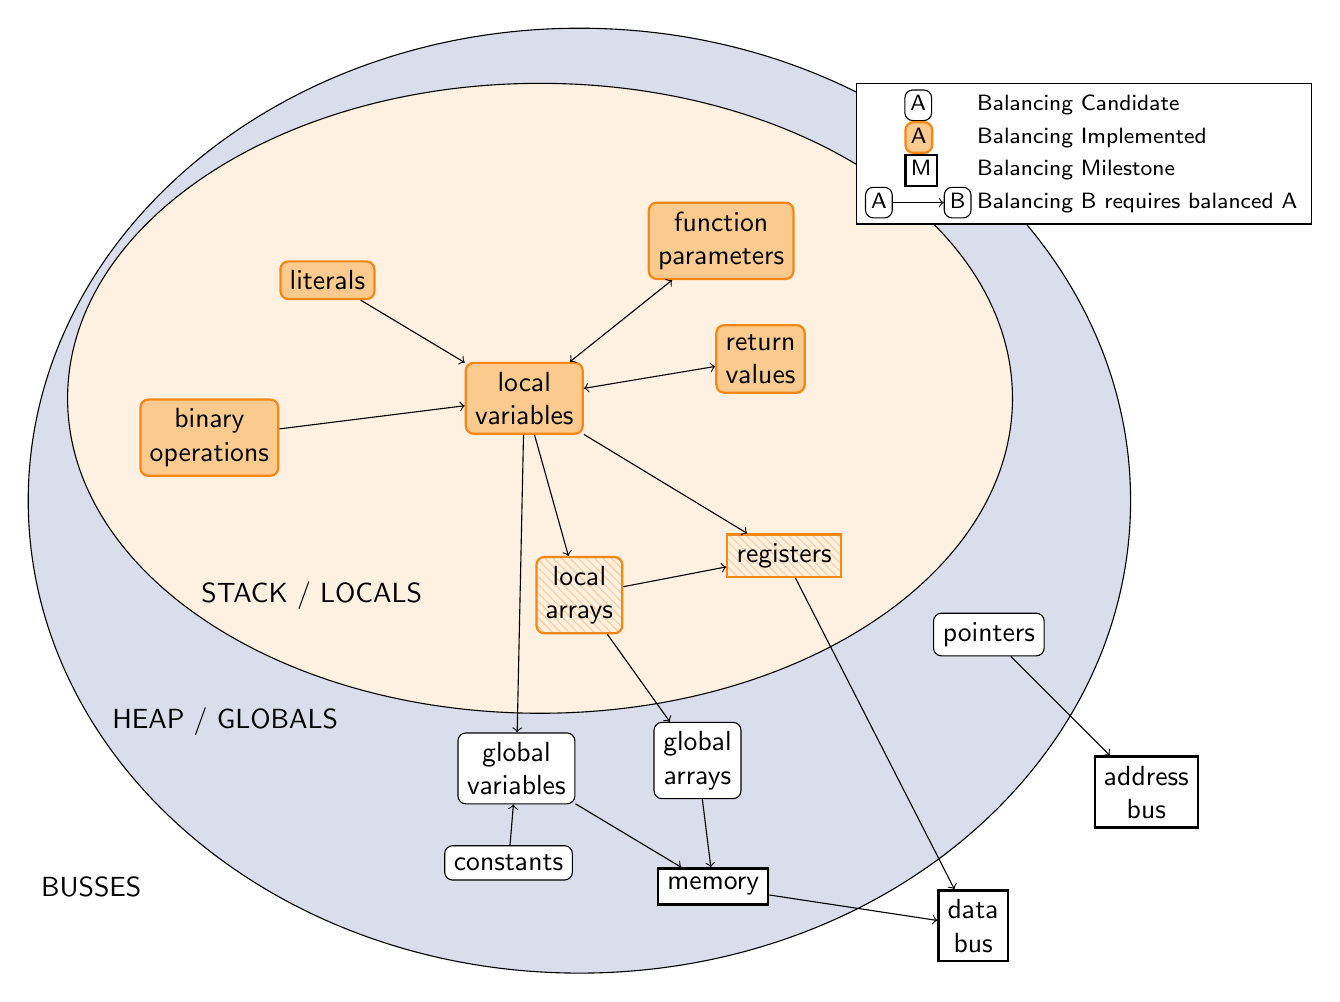
\begin{tikzpicture}
    \draw[fill=pantone289!10] (1.7, 0.7) ellipse (7cm and 6cm);
    \node[align=center] at (-2.8, -2.1) {HEAP / GLOBALS};

    \draw[fill=pantone144!10] (1.2,2) ellipse (6cm and 4cm);
    \node at (-1.7, -0.5) {STACK / LOCALS};

    \node at (-4.5, -4.2) {BUSSES};

    \node (literals) [candidate, balanced] at (-1.5,3.5) {literals};
    \node (ops) [candidate, balanced] at (-3,1.5) {binary \\ operations};
    \node (lvars) [candidate, balanced] at (1,2) {local \\ variables};
    \node (larrs) [candidate, todo] at (1.7,-0.5) {local \\ arrays};
    \node (params) [candidate, balanced] at (3.5, 4) {function \\ parameters};
    \node (returns) [candidate, balanced] at (4, 2.5) {return \\ values};
    \node (registers) [target, todo] at (4.3, 0) {registers};

    \draw[->] (literals) -> (lvars);
    \draw[->] (ops) -> (lvars);
    \draw[->] (lvars) -> (larrs);
    \draw[<->] (lvars) -> (params);
    \draw[<->] (lvars) -> (returns);

    \draw[->] (lvars) -> (registers);
    \draw[->] (larrs) -> (registers);

    \node (gvars) [candidate] at (0.9, -2.7) {global \\ variables};
    \node (garrs) [candidate] at (3.2, -2.6) {global \\arrays};
    \node (constants) [candidate] at (0.8, -3.9) {constants};
    \node (memory) [target] at (3.4, -4.2) {memory};
    \node (pointers) [candidate] at (6.9, -1.0) {pointers};

    \draw[->] (lvars) -> (gvars);
    \draw[->] (larrs) -> (garrs);
    \draw[->] (constants) -> (gvars);
    \draw[->] (gvars) -> (memory);
    \draw[->] (garrs) -> (memory);

    \node (databus) [target] at (6.7, -4.7) {data \\ bus};
    \node (addressbus) [target] at (8.9, -3.0) {address \\ bus};

    \draw[->] (registers) -> (databus);
    \draw[->] (memory) -> (databus);
    \draw[->] (pointers) -> (addressbus);

    \begin{customlegend}[legend cell align=left, legend entries={Balancing Candidate,Balancing Implemented, Balancing Milestone, Balancing B requires balanced A},
      %legend image post style={scale=2.3},
      legend style={at={(11,6)},font=\footnotesize}]
      \addlegendimage{legend image code/.code={\node[candidate] {A};}}
      \addlegendimage{legend image code/.code={\node[candidate, balanced] {A};}}
      \addlegendimage{legend image code/.code={\node[target] {M};}}
      \addlegendimage{legend image code/.code={\node[candidate] (A) at (-0.5, 0) {A};\node[candidate] (B) at (0.5,0){B}; \draw[->] (A) -> (B);}}
    \end{customlegend}
  \end{tikzpicture}
  \caption{Balancing dependencies in LLVM}
  \label{fig:balancing}
\end{figure}
\end{document}
